%Experimental Results and Analysis – in this section, you should show the quantitative results – charts and tables. Analyze the results by explaining and highlighting what is important on them in terms of your goals and what is bad. You should explain the strange results too.

%V ďalšej časti prezentujte vlastný prínos a vlastné výsledky porovnajte s výsledkami iných. Charakterizujte použité metódy.
%Vyhýbajte sa používaniu žargónu.
%Používajte starú múdrosť: 1 obrázok je viac než 1000 slov.

\subsection{Handwritten digits} 
\label{sec:results-digits} 

In this section, we wanted to test TLR on a high dimensional graphical task and compare it to other known models. For this we chose the \emph{handwritten digits} dataset (\ref{sec:datasets-digits}). As in the previous simulations, we trained the networks for range of $\lambda_v$ and $\lambda_h$ values to find best parameters. Then we analysed the network with best parameters individually. 

Before the training we splitted the dataset to \emph{train} set with 38,000 samples and \emph{test} set with 4,000 samples. Then we trained the networks on the train set and then evaluted them on the test set. The $Epoch_{\rm max}$ value was set to 20 and the training was stopped if $patSucc^F$ was not increased for 3 successive epochs. Architecture was 784--300--10 as it was used previously with BP. Note that for the final classification we chose the unit with greatest activation. 

%===============================================================
%===============================================================
%===============================================================
\subsubsection{Two learning rates} 
\label{sec:tlr-digits} 

We proved that TLR could learn high dimensional task as shown in figure~\ref{fig:results-tlr-digits-success}. The properties of the plot are similar to the 4-2-4 encoder case. It holds that $\lambda_h \ll \lambda_v$ and the success space is smooth. The main difference is the magnitude of values of both $\lambda_h$ and $\lambda_v$ is smaller. This notion indroduces a hypothesis that for \emph{higher} dimensional tasks, which usually also have more samples, \emph{lower} values of learning rates should be chosen. 

%[OLD]In comparison to TLR performances on tasks 4-2-4 encoder~(\ref{fig:results-tlr-auto4-performance}) and CBVA~(\ref{fig:results-tlr-k3-performance}) the successful values of $(\lambda_v,\, \lambda_h)$ were smaller. That introduces the hypothesis that the bigger set of samples, the lower the values of $(\lambda_v,\, \lambda_h)$. We suggest it as a possible future work in section~\ref{sec:future-work}. 

%Purpose: 
%======== (3D) L1 x L2 x patSuccF =========
%======== (3D) L1 x L2 x epochs =========
\begin{figure}[H]
  \centering
  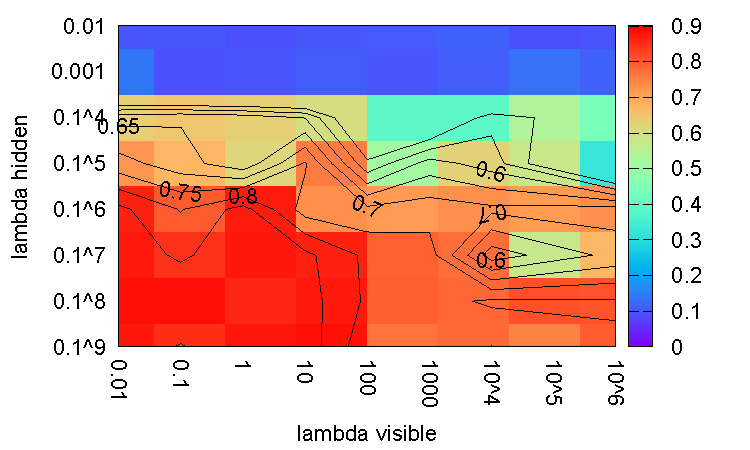
\includegraphics[width=0.60\textwidth]{img/tlr-digits-psf.pdf} %OPT add additional columns 
%  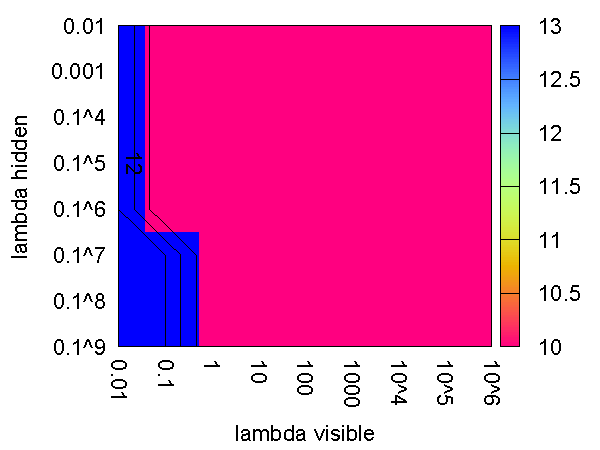
\includegraphics[width=0.49\textwidth]{img/tlr-digits-epoch.pdf}     
  \caption{TLR performance on the \emph{digits} task for $\sigma = 1/\sqrt{784+1} \approx 0.036$ and $\mu = 0.01$. Best $patSucc^F = 88.47\%$ with $\lambda_v=0.1$ and $\lambda_h=10^{-8}$.}
  \label{fig:results-tlr-digits-success}
\end{figure}


%======== (2D) best TLR on ALL_SUCC x epoch (std-dev) ==========
%\begin{figure}[H]
%  \centering
%  
\includegraphics[width=0.60\textwidth]{img/placeholder.png}   
%  \caption{TLR success rate timeline for the \emph{digits} task with $\sigma = 1/\sqrt{784+1}$, $\mu = 0.01$, $\lambda_v=0.1$ and $\lambda_h=10^{-8}$.}
%  \label{fig:results-tlr-digits-epoch} 
%\end{figure}

%===============================================================
%===============================================================
%===============================================================
\subsubsection{Comparison} 
\label{sec:results-cmp-digits} 

For comparison of TLR on the \emph{digits} task we chose neural network models with similar architecture from \citet{digits2014mnist}. From table~\ref{tab:results-cmp-digits} we see that TLR is able to learn higher dimensional tasks, but still has a performance gap to fill. Note that it performs comparably as \emph{linear classifier}, i.e.~a~two layer neural network. 

\begin{table}[H] 
  \centering
    \begin{tabular}{|l|l|l|l|l|}
    \hline
    Algorithm (section)&$\lambda_h$&$\lambda_v$&$patSucc^F$ &Epochs\\ %&SEM(success) \\
    \hline
    Linear classifier & -- & -- & 88 & -- \\ 
    \hline
    BP 784--300--10~(\ref{sec:models-bp})& -- & -- & 95.3 & -- \\ 
    \hline 
    BAL 784--300--10~(\ref{sec:models-bal})& 0.01 & 0.01 & 9.8 & 20 \\
    \hline 
    TLR 784--300--10~(\ref{sec:models-bp})& $10^{-8}$ & 0.1 & 88.47 & 20 \\
    \hline 
    GeneRec 784--300--50--10~(\ref{sec:sim-our-generec-multi})& 0.03 & 0.03 & 43.22 & 50 \\
    \hline 
    \end{tabular}
  \caption{Comparison of different models on the \emph{digits} task. Data from \citet{lecun1998gradient} and \citet{digits2014mnist}.} 
  \label{tab:results-cmp-digits}
\end{table}

%===============================================================
%===============================================================
%===============================================================
\subsubsection{Backward representations} 
\label{sec:our-backward-repre}

The goal of \emph{backward representations} for \emph{heteroassociative} tasks, i.e.~tasks which have multiple inputs for the same output, is to \emph{depict} the backward activation of an particular output. In case of BAL~(\ref{sec:models-bal}), the backward representations are all possible values of $x^{\rm B}$ for each possible output value $y^{\rm B}$, i.e.~target. For example the backward representation of digit "8" in TLR~(\ref{sec:our-tlr}) is show in figure~\ref{fig:our-backward-repre-8}. This is image is generated by clamping vector $(0000000100)$ to the output layer, then doing a backward pass and depicting the activation on the input layer. 

\begin{figure}[H]
  \centering
  
\includegraphics[width=0.2\textwidth]{img/tlr-digit-8.png} 
  \caption{Backward representation of digit "8" in TLR.}
  \label{fig:our-backward-repre-8}
\end{figure}

As we can see in figure~\ref{fig:results-tlr-digits-backward}, TLR gives us readable backward activations. This intuitively proves that the model is capable of bidirectional training. The shapes could be best seen for digits ''0'', ''1'' and ''8''. By using some imagination we can also see the other digits. 

%======== (2D) for best network vs. sample digits
\begin{figure}[H]
  \centering
  
\includegraphics[width=0.98\textwidth]{img/tlr-digits.png}    
  \caption{Backward representations for the most successful TLR instance on the \emph{digits} task.}
  \label{fig:results-tlr-digits-backward} 
\end{figure}
